\subsection{Analisi FEM conduzione stazionaria}
Si misura la resistenza di un fluido attraversato da corrente.
\begin{figure}[H]
\centering
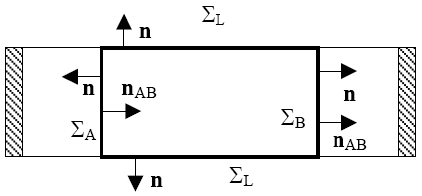
\includegraphics[width=0.4\linewidth]{conduzione_FEM}
\end{figure}
Si ricordano le ipotesi di solenoidalità di $\vec{J}$ e conservatività di $\vec{E}$
\begin{align*}
\oint_\gamma \vec{E}\cdot\hat{t} dl = 0 &\qquad \forall\ \gamma \\
\oiint_\Sigma \vec{J}\cdot\hat{n} dS = 0 &\qquad \forall\ \Sigma
\end{align*}
Si consideri una linea che unisca i due elettrodi, la scelta non è importante
essendo il campo $\vec{E}$ conservativo.
La componente normale alla superficie laterale è nulla a causa dell'isolamento
dell'aria mentre i flussi attraverso le superfici $\Sigma_A$ e $\Sigma_B$ sono 
uguali e opposti, o identici a seconda di come si considerano le normali alle 
superfici, in conclusione si può dire che la corrente che attraversa la superficie $A$
è identica a quella che attraversa la superficie $B$.

Il modello differenziale in analisi è il seguente
\begin{align*}
&\nabla\times\vec{E} = 0 \Rightarrow \vec{E} = -\nabla U\\
&\nabla\cdot\vec{J} = 0 \Rightarrow \nabla^2 U = 0 \quad \text{con }\vec{J} = \sigma\vec{E}\\
&U|_{l_1}  = V_1\\
&U|_{l_2} = 0 \\
&\left.\frac{\partial U}{\partial \hat{n}}\right|_{l_3 \cup l_4} =0
\end{align*}

Si esegue lo strumento \textit{pdetool} e si definisce una geometria rettangolare,
si impostano le condizioni di Dirichlet alle superfici degli elettrodi e Neumann a quelle 
laterali.
In PDE Mode si imposta l'equazione ellittica con costanti unitarie, si imposta il meshing
è si calcola la soluzione.
Per calcolare la resistenza si può esportare la mesh e calcolare l'intensità di corrente su 
una faccia.
Per calcolare l'intensità di corrente occorre dunque integrare il flusso della densità
di corrente per la superficie di frontiera.
La superficie è discretizzata, vanno quindi considerati i singoli triangoli
che compongono la superficie laterale, si approssima la derivata al rapporto incrementale,
preso un punto sull'ascissa $x=0$ e ordinata $y$, si sa con certezza che ha potenziale 
unitario perché imposto dal problema, resta quindi da stimare il potenziale nel 
punto $(x+\Delta x,y)$ per calcolarne la derivata
$$
\frac{V(x+\Delta x,y) - V (0,y)}{\Delta x}\simeq \frac{\partial V}{\partial x} (0,y) +o(\Delta x^2)
$$
Sfruttando il comando ``tri2grid'' è possibile interpolare una mesh triangolare
in una griglia rettangolare riportando i valori corretti
\begin{lstlisting}[style=Matlab-editor,language = Matlab]
%plot mesh
figure();
pdemesh(p,e,t);
%definizione ascissa di controllo
dx = 0.1;
x = dx*ones(20,1)-0.5;
y = linspace(0,0.5,20);
%Plot della linea di controllo sulla mesh, colore magenta
hold on;
plot(x,y,'m');
%Interpolazione della mesh
u_dx = tri2grid(p,t,u,x,y);
%Calcolo rapporto incrementale rispetto al potenziale 1 di partenza
du_dx = (u_dx-1)/dx;
Ex = -du_dx;
%Media del campo
mean(Ex)
%Conducibilita' e densita' di corrente
gamma = 1;
Jx = gamma*Ex
%Dimensioni conduttore
h = 0.5;
Lz = 1;
S = h * Lz;
%Stima della corrente
i = mean(mean(Jx))*S
\end{lstlisting}
È possibile ripetere l'analisi per un conduttore emisferico interrato e confrontarla
con la resistenza analitica.
